%----------------------------------------------------------
% Fichier: rapport.tex    Auteur(s): Simon DÉSAULNIERS
% Date: 2013-04-28
%----------------------------------------------------------
% Rapport du Travail de Session du cours SMI1002 de
% l'Université du Québec à Trois-Rivières.
%----------------------------------------------------------
\documentclass[11pt,french]{article}

\usepackage[frenchb]{babel}
\usepackage[utf8]{inputenc}
\usepackage[T1]{fontenc}

\usepackage{graphicx}

\usepackage{hyperref}
\hypersetup{hidelinks}

% Style des pages
\usepackage{fancyhdr}
\pagestyle{fancy}
\lhead{Travail de Session}

% Caractères mathématiques
\usepackage{amssymb}

\usepackage{color}

\usepackage{textpos}

\usepackage[final]{pdfpages}

% Affichage de code source
\usepackage{listings}
\definecolor{dkgreen}{rgb}{0,0.6,0}
\definecolor{dkblue}{rgb}{0,0,0.8}
\definecolor{gray}{rgb}{0.5,0.5,0.5}
\definecolor{mauve}{rgb}{0.58,0,0.82}

\usepackage{courier}

\lstset{ %
backgroundcolor=\color{white},   % choose the background color; you must add \usepackage{color} or \usepackage{xcolor}
basicstyle=\footnotesize,        % the size of the fonts that are used for the code
breakatwhitespace=false,         % sets if automatic breaks should only happen at whitespace
breaklines=true,                 % sets automatic line breaking
captionpos=b,                    % sets the caption-position to bottom
commentstyle=\color{dkblue},    % comment style
deletekeywords={...},            % if you want to delete keywords from the given language
escapeinside={\%*}{*)},          % if you want to add LaTeX within your code
extendedchars=true,              % lets you use non-ASCII characters; for 8-bits encodings only, does not work with UTF-8
frame=single,                    % adds a frame around the code
keywordstyle=\color{dkgreen},       % keyword style
morekeywords={*,...},            % if you want to add more keywords to the set
numbers=left,                    % where to put the line-numbers; possible values are (none, left, right)
numbersep=5pt,                   % how far the line-numbers are from the code
numberstyle=\tiny\color{gray}, % the style that is used for the line-numbers
rulecolor=\color{black},         % if not set, the frame-color may be changed on line-breaks within not-black text (e.g. comments (green here))
showspaces=false,                % show spaces everywhere adding particular underscores; it overrides 'showstringspaces'
showstringspaces=false,          % underline spaces within strings only
showtabs=false,                  % show tabs within strings adding particular underscores
stepnumber=2,                    % the step between two line-numbers. If it's 1, each line will be numbered
stringstyle=\color{red},     % string literal style
tabsize=2,                       % sets default tabsize to 2 spaces
xleftmargin=\parindent,
title=\lstname                   % show the filename of files included with \lstinputlisting; also try caption instead of title
}


\newcommand{\HRule}{\rule{\linewidth}{0.5mm}}


\begin{document}
    % PAGE TITRE
    \begin{titlepage}
        \begin{center}
    
            
\includegraphics[height=3cm]{./aux/bd1.png}
            \\[3cm]
            
            \textsc{\LARGE Base de Données II}
            \\[0.2cm]
            \textsc{\Large SMI1002}
            \\[2cm]
            \HRule \\[0.5cm]
            {\huge \bfseries Travail de Session}
            \HRule \\[2cm]
            Par\\
            Simon Désaulniers\\
            Daniel St-Pierre

            \vfill
            2013-04-28\\
            Université du Québec à Trois-Rivières
            \thispagestyle{empty}
        \end{center}
    \end{titlepage}
    \newpage
    
    % TABLE DES MATIÈRES
    \pagenumbering{roman}
    \setcounter{page}{1}
    \tableofcontents
    \newpage

    % CORPS DU RAPPORT
    \pagenumbering{arabic}
    \setcounter{page}{1}

    \section*{Introduction} % (fold)
    \label{sec:Introduction}
        \subsection*{But} % (fold)
        \label{sub:but}
            Le travail de session du cours SMI1002 vise à maîtriser la programmation d'une base
            de données avec gestion de la concurence de requêtes, l'élaboration de requêtes optimisées
            et la gestion de panne de matériel.
        % subsection but (end)
        \subsection*{Mise contexte} % (fold)
        \label{sub:mise-en-contexte}
            L'association LAN-UQTR a pour but d'organiser un événement annuel à l'UQTR destiné autant aux
            étudiants de l'UQTR que les résidents de la région de la mauricie et ses alentours. L'événement
            consiste en un rassemblement d'autour de 200 personnes dans une ou plusieurs salles à l'Université
            du Québec à Trois-Rivières pour une période de 48 heures. Les gens y participant apportent leur matériel
            informatique pour le brancher en réseau avec le reste des participants. Par la suite, ils jouent de façon
            libre avec les autres ou participent à différents tournois de jeux connus.\\

            L'organisation d'une telle activité nécessite de la préparation de quelques mois à l'avance afin de faire
            le plan des tournois organisés, les jeux disponibles et la liste des billets vendus. L'association LAN-UQTR
            a donc besoin d'un système informatique muni d'une base de données faisant la gestion du personnel, des joueurs,
            des équipes de jeux et des tournois lors de l'événement.
        % subsection mise-en-contexte (end)
    % section Introduction (end)
    \newpage

    \section{Conception UML} % (fold)
    \label{sec:concep-uml}
        La conception de la base de données est faite par un diagramme de type UML. Selon les différents besoins venant
        de la situation, on peut tirer un sous-ensemble de ceux-ci consistant en un cas indéndant. Nous avons décidé
        d'utiliser le cas du concept d'{\bf événement}, de {\bf tournoi}, de {\bf jeu} et de {\bf type de jeu}. Le diagramme résultant est le suivant:
        \begin{center}
            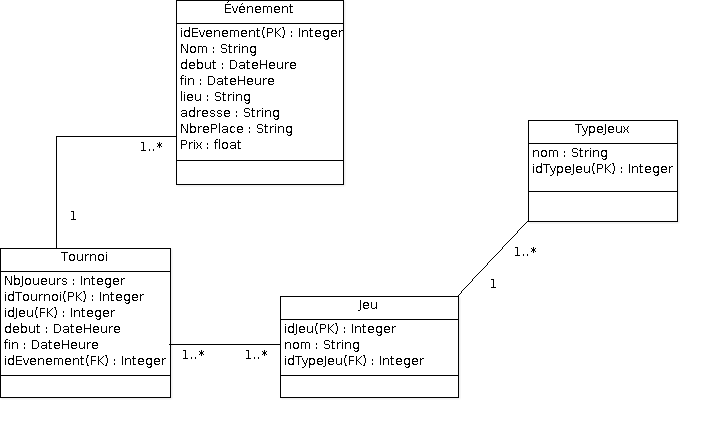
\includegraphics[width=12cm]{../../conception/DiagrammeUML-simdan.png}
        \end{center}

        \subsection{Table Événement} % (fold)
        \label{sub:table-enevement}
            Cette table représente un événement annuel organisé. Il possède les champs suivants:\\
            \begin{itemize}
                \item {\bf idEvenement}: Clé primaire de la table.
                \item {\bf Nom}: Le nom de l'événement (p. ex: \emph{Lan Party 2013 à l'UQTR}).
                \item {\bf debut}: Date et l'heure de début de l'événement.
                \item {\bf fin}: Date et l'heure de fin de l'événement.
                \item {\bf lieu}: Endroit où aura lieu l'événement.
                \item {\bf adresse}: L'adresse précise où aura lieu l'événment.
                \item {\bf NbrePlace}: Le nombre de places disponibles à la participation de cet événement.
                \item {\bf Prix}: Le prix à payer afin de participer à cet événement.
            \end{itemize}

            \subsubsection{Relations} % (fold)
            \label{ssub:relation-evenement}
                La table possède une seule relation. Celle-ci est entre la table événement et Tournoi. La cardinalité de cet relation
                est d'aucun à plusieurs (0..*) du point de vue de la table événement puisqu'un événement possède de un à plusieurs tournoi
                à son actif.
            % subsubsection Relations (end)
        % subsection Table Événement (end)
        \subsection{Table Tournoi} % (fold)
        \label{sub:table-tournoi}
            La table Tournoi représente un tournoi organisé lors d'un événement. Ce tournoi est une compétition à savoir quel joueur
            donne la meilleure performance au jeu vidéo faisant l'objet du tournoi. Les attributs sont les suivants:\\
            \begin{itemize}
                \item {\bf idTournoi}: Clé primaire de la table.
                \item {\bf idJeu}: Clé étrangère de la table Jeu car à un tournoi est associé un jeu.
                \item {\bf idEvenement}: Clé étrangère de la table Événement car pour un tournoi, on a un événement associé.
                \item {\bf NbreJoueurs}: Le nombre de joueurs admissible au tournoi.
                \item {\bf debut}: La date et l'heure précise du début du tournoi.
                \item {\bf fin}: La date et l'heure précise de la fin du tournoi.
            \end{itemize}

            \subsubsection{Relations} % (fold)
            \label{ssub:relations-tournoi}
                Il y a deux relations se trouvant entre la table Tournoi et deux autres tables:\\

                \begin{itemize}
                    \item Il y a une relation entre la table tournoi et événement puisqu'un tournoi est nécessairement organisé lors
                        d'un événement. On a une cardinalité de un à un puisqu'un tournoi à une certaine date est organisé qu'à un seul
                        événement.
                    \item La table jeu est liée à la table Tournoi puisqu'un tournoi porte nécessairement sur un jeu. Du côté de la table
                        Tournoi, la cardinalité est 1 puisqu'un tournoi ne porte que sur un seul jeu.
                \end{itemize}
            % subsubsection relations-tournoi (end)
        % subsection table-tournoi (end)
        \subsection{Table Jeu} % (fold)
        \label{sub:table-jeu}
            La table jeu consiste en l'ensemble des jeux vidéos qui seront supportés pour jouer durant l'événement. On compte donc les champs
            suivants:
            \begin{itemize}
                \item {\bf idJeu}: Clé primaire de la table.
                \item {\bf idTypeJeu}: Clé étrangère venant de la table TypeJeu.
                \item {\bf nom}: Le nom du jeu vidéo en question.
            \end{itemize}
            \subsubsection{Relations} % (fold)
            \label{ssub:relations-jeu}
                Il existe deux relations mettant en jeu cette table:
                \begin{itemize}
                    \item Une table Jeu possède une relation avec un table tournoi puisqu'un jeu est joué dans un ou plusieurs tournois (1..*)
                    \item La table TypeJeu est aussi en relation avec la table jeu puisqu'un jeu appartient nécessairement à un type de jeu.
                \end{itemize}
            % subsubsection relations-jeu (end)
        % subsection table-jeu (end)
        \subsection{Table TypeJeu} % (fold)
        \label{sub:table-type-jeu}
            C'est une façon de catégoriser les jeux vidéos. Par exemple, le jeu vidéo {\it Starcraft 2} 
            est de la catégorie des jeux de stratégie en temps réel. Dans la table, on retrouve les champs suivants:
            \begin{itemize}
                \item {\bf idTypeJeu}: La clé primaire de la table.
                \item {\bf nom}: Le nom du type de jeu.
            \end{itemize}
            \subsubsection{Relations} % (fold)
            \label{ssub:relations-type-jeu}
                La table TypeJeu est en relation avec un jeu puisqu'un Type de jeu a au moins un jusqu'à plusieurs jeu dans sa catégorie (1..*).
            % subsubsection relations-type-jeu (end)
        % subsection table-type-jeu (end)
    % section concep-uml (end)
    \newpage
    \section{Optimisation de requêtes} % (fold)
    \label{sec:optimisation-requetes}
        Parmis les requêtes SQL que l'interface que notre programme offre, nous en avons choisi une qui était susceptible d'être optimisée:
        $$\Pi_{idJoueur,nom,gamertag,courriel,sexe,datenaissance}$$
        $$\Bigg |$$
        $$\sigma_{idJoueur=ID}$$
        $$\Bigg |$$
        $$\rhd \lhd_{idJoueur}$$
        \begin{textblock}{0.2}(4.2,0)
            
\includegraphics[height=2cm]{aux/ligneDiag.png}
        \end{textblock}
        \begin{textblock}{0.2}(3.2,0)
            
\includegraphics[height=2cm]{aux/ligneDiag2.png}
        \end{textblock}

        \vspace{1.8cm}

        $$JOUEUR \ \ \ JOUEUREQUIPE$$

        \vspace{1.5cm}
        
        On optimise cette requête en utilisant l'heuristique suivant:
        \begin{quotation}
            \og \emph{Effectuer la sélection le plus tôt possible.} \fg
        \end{quotation}
        
        \newpage
        De cette façon, on peut obtenir le résultat suivant:
       
        $$\Pi_{idJoueur,nom,gamertag,courriel,sexe,datenaissance}$$
        $$\Bigg |$$
        $${} \times {}$$
        \begin{textblock}{0.2}(4.2,0)
            
\includegraphics[height=2cm]{aux/ligneDiag.png}
        \end{textblock}
        \begin{textblock}{0.2}(3.2,0)
            
\includegraphics[height=2cm]{aux/ligneDiag2.png}
        \end{textblock}

        \vspace{1.8cm}

        $$\sigma_{idJoueur=ID} \ \ \ \sigma_{idJoueur=ID}$$
        $$\Bigg | \ \ \ \ \ \ \ \ \ \ \ \ \ \ \ \ \ \ \ \ \ \ \ \ \Bigg |$$
        $$JOUEUR \ \ \ \ \ JOUEUREQUIPE$$
    % section optimisation-requetes (end)
    \section{Journal} % (fold)
    \label{sec:Journal}
        Un journal gardant la trace des requêtes a été mis en place et chaque transaction est enregistrée dans un fichier.
    % section Journal (end)
    \section*{Conclusion} % (fold)
    \label{sec:Conclusion}
        Finalement, ce travail permet de remarquer l'attention nécessaire à porter à l'ordonnencement des opérations d'algèbre relationnel
        représentant la requête faite au système de gestion de base de données.
    % section Conclusion (end)
\end{document}
